%%%%%%%%%%%%%%%%%%%%%%%%%%%%%%%%%%%%%%%%%%%%%%%%%%%%%%%%%%%%%%%%%%%
%                                                                 %
%  GEANT manual in LaTeX form                              %
%                                                                 %
%  Michel Goossens (for translation into LaTeX)                   %
%  Version 1.00                                                   %
%  Last Mod. Jan 24 1991  1300   MG + IB                          %
%                                                                 %
%%%%%%%%%%%%%%%%%%%%%%%%%%%%%%%%%%%%%%%%%%%%%%%%%%%%%%%%%%%%%%%%%%%
\Origin{R.Brun}
\Submitted{01.11.83}    \Revised{15.12.93}
\Version{Geant 3.16}    \Routid{TRAK499}
\Makehead{The space point data structure JXYZ}

\begin{figure}[hbt]
     \centering
     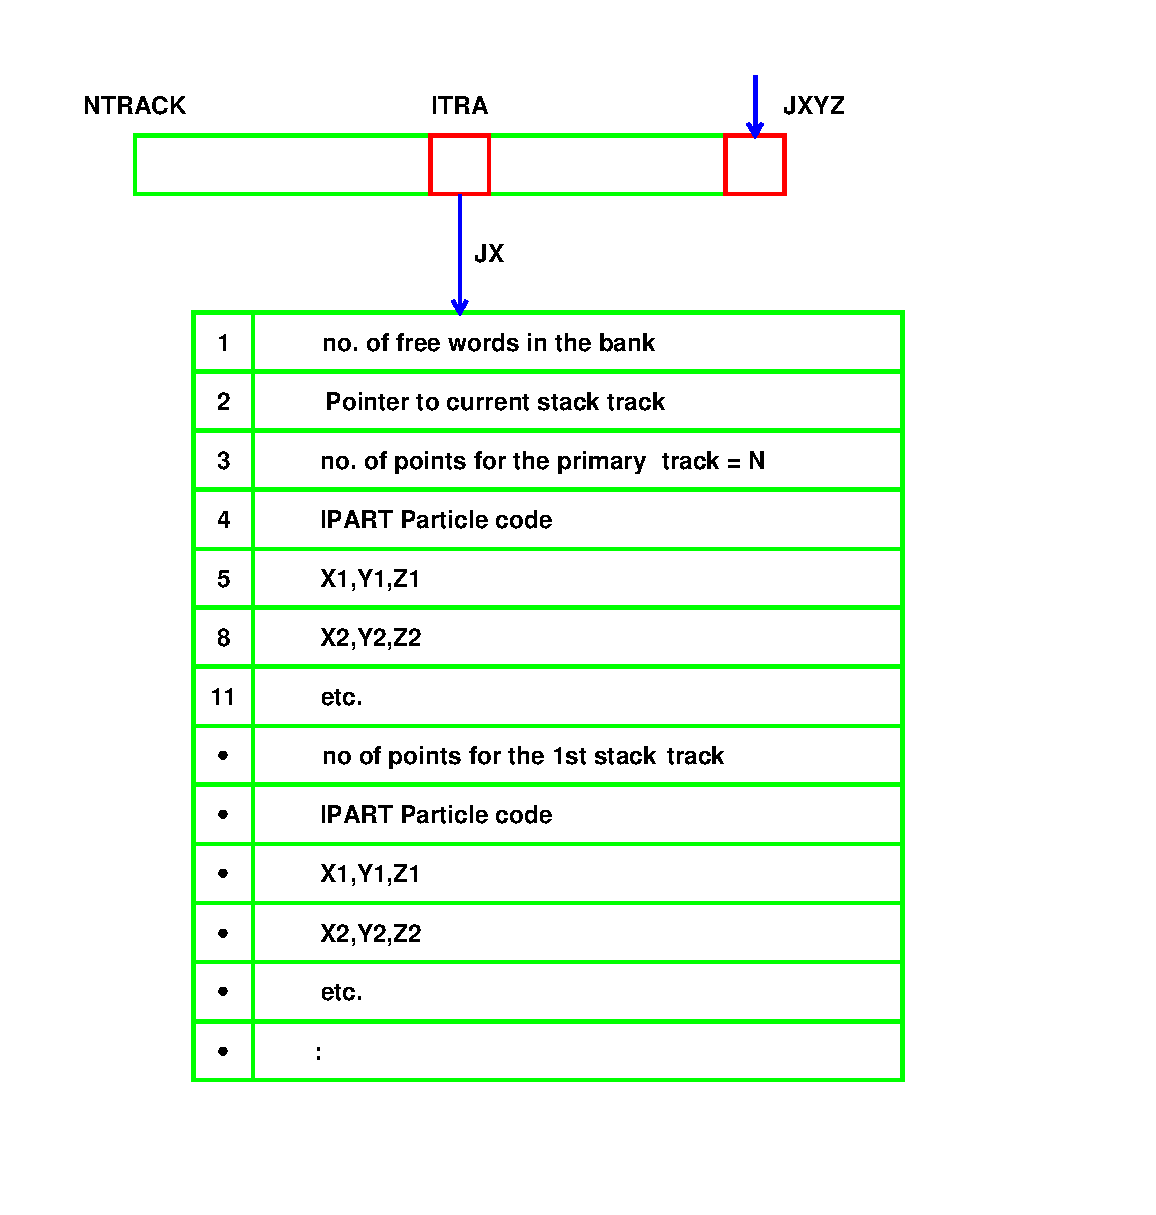
\epsfig{file=eps/trak499-1.eps,width=14cm}
     \caption{Layout of the {\tt JXYZ} data structure}
     \label{fg:trak499-1}
\end{figure}

{\tt JX=LQ(JXYZ-ITRA)} is the pointer to the space points of track number 
{\tt ITRA}
 
The space point banks {\tt JXYZ} are only used for debug and display
purposes. They can be filled by using the routine \Rind{GSXYZ} from
\Rind{GUSTEP}. The drawing routine \Rind{GDXYZ}
gets the space coordinates from {\tt JXYZ}.
